\documentclass{beamer}

\usepackage{graphics}
\usepackage{graphicx}
\usepackage{hyperref}
\usepackage[latin1]{inputenc}

\usepackage{listings}
\lstset{showstringspaces=false,frame=trBL,frameround=tttt,tabsize=8,basicstyle=\tiny,breaklines=true,breakatwhitespace=true}
\lstdefinestyle{bash}{language=bash}
\lstdefinestyle{Perl}{language=Perl}
\lstdefinestyle{C++}{language=C++}
\lstdefinestyle{DTD}{language=XML}
\lstdefinestyle{XML}{language=XML,usekeywordsintag=false,markfirstintag=true}
\newcommand{\includecode}[2]{\lstinputlisting[style=#1]{#2}}
%\lstnewenvironment{code}{}{}
\lstnewenvironment{code_bash}{\lstset{style=bash}}{}
\lstnewenvironment{code_perl}{\lstset{style=Perl}}{}
\lstnewenvironment{code_cpp}{\lstset{style=C++}}{}
\lstnewenvironment{code_dtd}{\lstset{style=DTD}}{}
\lstnewenvironment{code_xml}{\lstset{style=XML}}{}

\newcommand{\textcode}[1]{{\small {\tt #1}}}

% ---- format de page A4
% 	\setlength{\textwidth }{16cm}	% largeur de ligne
% 	\setlength{\textheight}{23cm}   % hauteur du texte
	\setlength{\oddsidemargin}{-17mm} % marge pages impaires
	\setlength{\evensidemargin}{-17mm}% marge pages paires
% 	\setlength{\topmargin}{0cm} 	
% 	\setlength{\headheight}{14pt} 
% 	\setlength{\headsep}{0.5cm} 

\title[Introdution to SOFA]{An Introduction to Sofa}
\author[Faure]{%
  Fran�ois~Faure\inst{1} }
\institute[Univ. Grenoble]{
  \inst{1}%
  Grenoble Universities\\
  INRIA - Evasion
  }
\date[September 2007]{September 11th 2007}
\subject{Computational Sciences}


\begin{document}

  \frame
  {
    \titlepage
  }

%\section{Overview}

\begin{frame}
 \frametitle{SOFA - Simulation Open Framework Architecture}
\begin{itemize}
 \item Open Source framework primarily targeted at real-time simulation
\begin{itemize}
 \item create complex and evolving simulations by combining new algorithms with algorithms already included in SOFA
  \item modify most parameters of the simulation: deformable behavior, surface representation, solver, constraints, collision algorithm, etc. by simply editing an XML file
 \item build complex models from simpler ones using a scene-graph description
 \item efficiently simulate the dynamics of interacting objects using abstract equation solvers
 \item reuse and easily compare a variety of available methods 
\end{itemize}
\item Currently developed by four research teams in two institutes: INRIA(Alcove, Asclepios, Evasion),  CIMIT(SimGroup,MIT/Harvard/MGH)
%\item 15 developers, 30 users
\end{itemize}
\end{frame}

\begin{frame}
 \frametitle{Main Features}
\begin{itemize}
 \item High modularity using a scene graph
 \item Multiple models of the same object can be synchronized using mappings
 \item Current implementations:
\begin{itemize}
 \item deformable objects (springs, FEM)
 \item rigid bodies (6-dof) 
 \item fluids (SPH, Eulerian)
 \item collision detection: spheres, triangles
 \item explicit and implicit time integration
\end{itemize}

\end{itemize}
\end{frame}


\begin{frame}
 \frametitle{Using Sofa}
\begin{itemize}
 \item In your application, as an external simulation library (C++, LGPL license)
 \item As a stand-alone application with one of the default user interfaces (Qt,Glut) and renderers (OpenGL, Ogre)
\begin{figure}
 \centering
 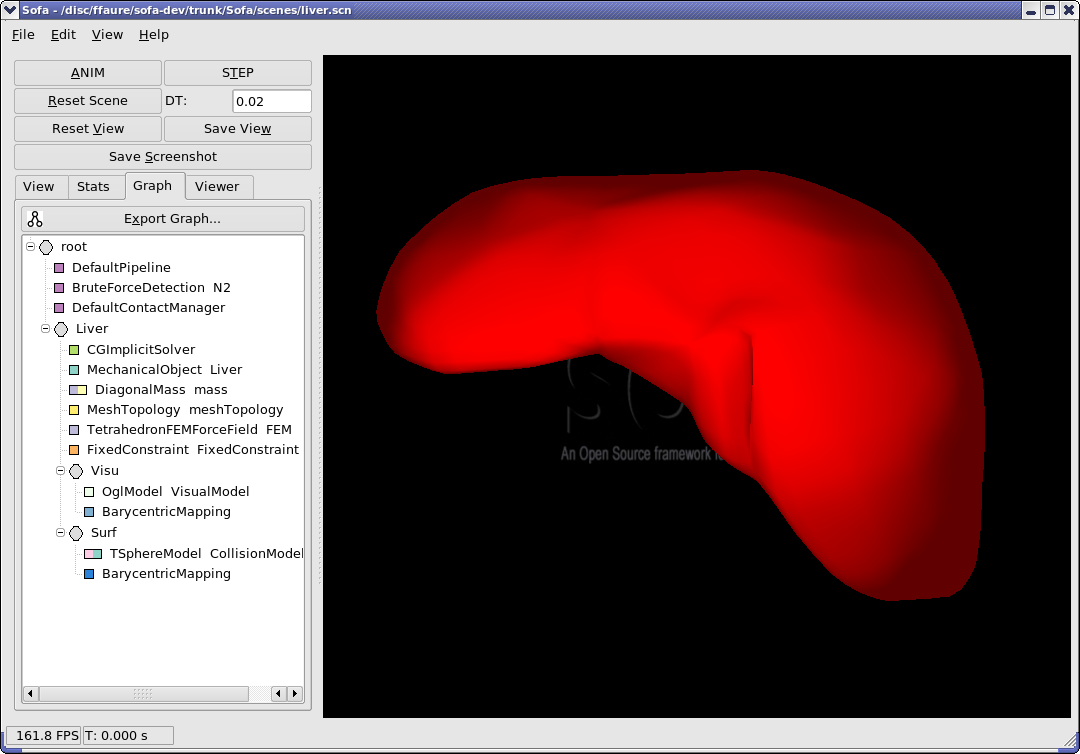
\includegraphics[width=0.7\linewidth]{sofa-window.png}
 % sofa-window.png: 161083904x0 pixel, 0dpi, infxnan cm, bb=
 \caption{Sofa stand-alone with Qt GUI and OpenGL rendering.}
 \label{fig:sofa-window}
\end{figure}

\end{itemize}

\end{frame}


\begin{frame}
 \frametitle{Data structure}
Scene graph with three levels of hierarchy
\begin{itemize}
 \item Nodes contains Nodes and Components.
 \item Components are leaves of the scene graph. They implement algorithms. They contain DataFields.
\item DataFields contain raw data (positions, masses, ...)
\end{itemize}
Example: A mass-spring string and a rigid body
\begin{figure}
\newcommand{\heigh}{25mm}
\begin{tabular}{ccc}
\begin{tabular}{c}
 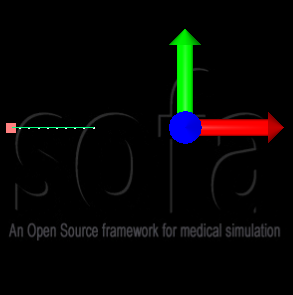
\includegraphics[height=\heigh]{mixed1.png} \\ the objects: \\ one string\\on rigid
\end{tabular}
&
\begin{tabular}{c}
 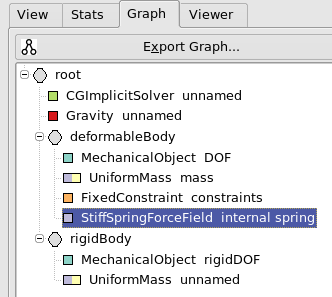
\includegraphics[height=\heigh]{mixed3.png} \\ scene graph: \\ 3 nodes\\8 components 
\end{tabular}
&
\begin{tabular}{c}
 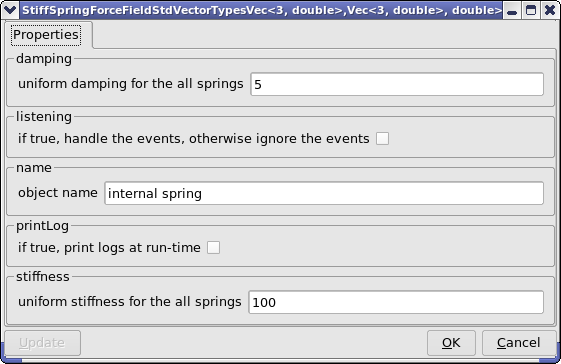
\includegraphics[height=\heigh]{mixed4.png} \\ the datafields of a\\ selected component \\
\end{tabular}
\end{tabular}
\end{figure}

\end{frame}


\begin{frame}
\frametitle{Why using scene graphs}
\begin{itemize}
 \item standard graphics tool 
\begin{itemize}
 \item modeling languages: VRML1, VRML2, X3D...
 \item libraries: OpenInventor, Java3D, OpenSG, OpenSceneGraph,...
\end{itemize}
\item simple structure (Directed Acyclic Graph): no cyclic dependencies 
\item abstraction and modularity
 \item dynamically add or remove objects in the scene
 %\item replacing a component while leaving the others unchanged
 \item I/O file format
\end{itemize}
\end{frame}

\begin{frame}
 \frametitle{Multiple models of a given object}
\begin{columns}
 \column{0.5\linewidth}
\begin{itemize}
 \item different geometries for different purposes
 \item one master geometry (mechanical behavior) contains the independent degrees of freedom (dof)
 \item implemented as a node hierarchy
 \item non-independent dofs updated using \emph{mappings}
\end{itemize}

 \column{0.5\linewidth}
\begin{figure}
 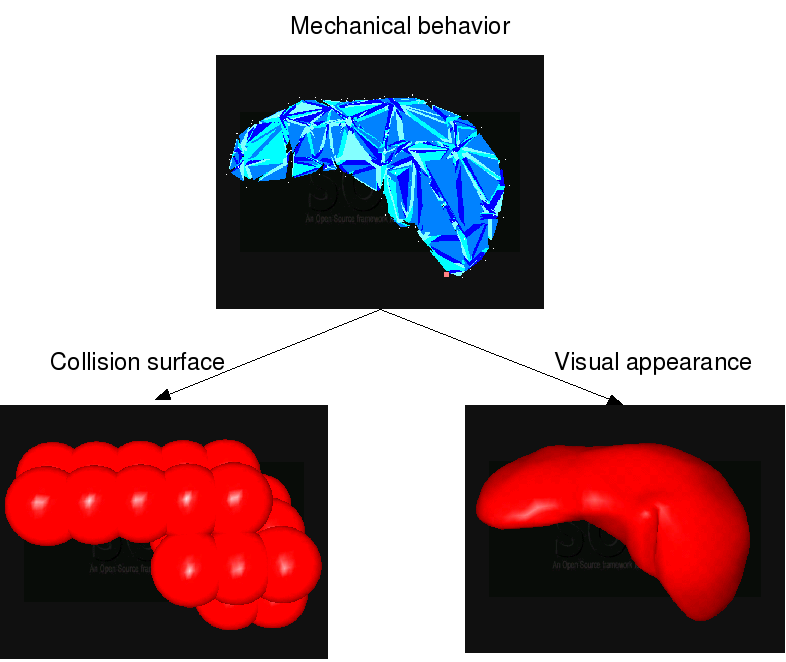
\includegraphics[width=\linewidth]{slides-fig-multimodal.png}
\end{figure}

\end{columns}
\end{frame}



\begin{frame}
 \frametitle{Example of mapping}
\begin{columns}
 \column{0.6\linewidth}
\begin{itemize}
 \item 4 mechanical control points
 \item one finite element (tetrahedron)
 \item hundreds of vertices in the visual model, all totally defined by the mechanical control points
\end{itemize}
\begin{tabular}{c}
 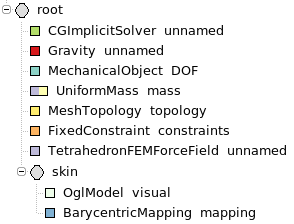
\includegraphics[width=\linewidth]{mixed7.png}
\end{tabular}

 \column{0.4\linewidth}
\begin{figure}
\begin{tabular}{c}
 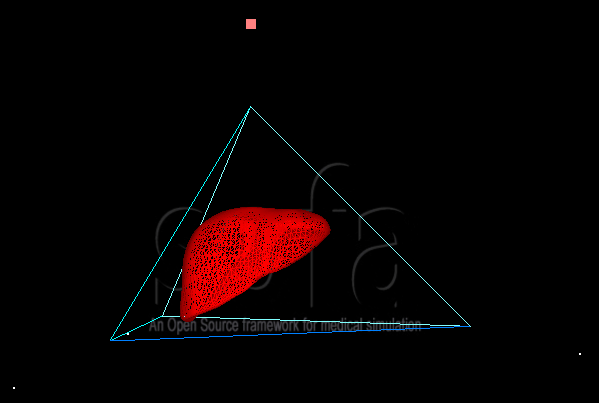
\includegraphics[width=\linewidth]{mixed5.png}\\
 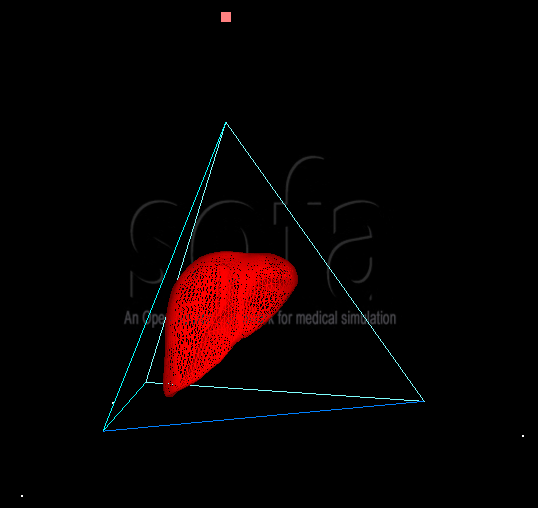
\includegraphics[width=\linewidth]{mixed6.png}
\end{tabular}
\end{figure}

\end{columns}
\end{frame}

\begin{frame}
 \frametitle{Modularity: various mechanical models attached to the same collision model}
\begin{figure}
 \centering
 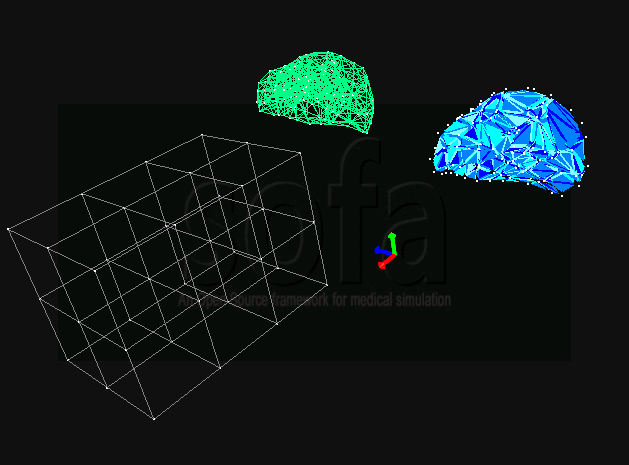
\includegraphics[width=0.4\linewidth]{demoLiverFall1.png}
 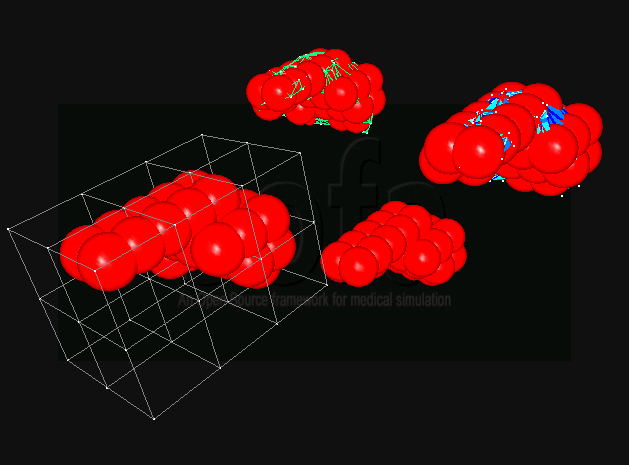
\includegraphics[width=0.4\linewidth]{demoLiverFall2.png}
 % demo.: 1179666x1179666 pixel, 0dpi, infxinf cm, bb=
\end{figure}
\begin{itemize}
 \item different mechanical models
 \item same collision model attached using the appropriate mapping 
\end{itemize}
\end{frame}

\begin{frame}
 \frametitle{Modularity: various collision models attached to the same mechanical model}
\begin{figure}
 \centering
 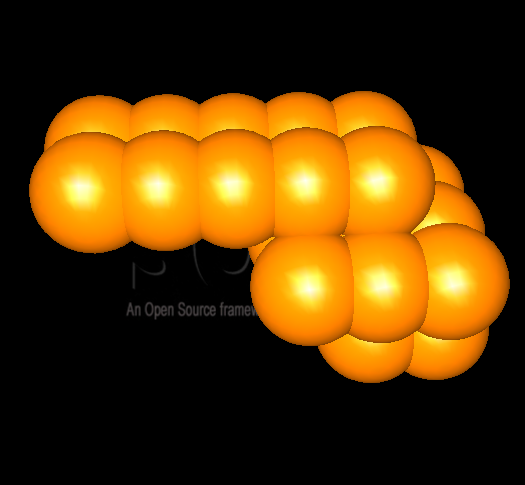
\includegraphics[width=0.4\linewidth]{liver_collision_spheres.png}
 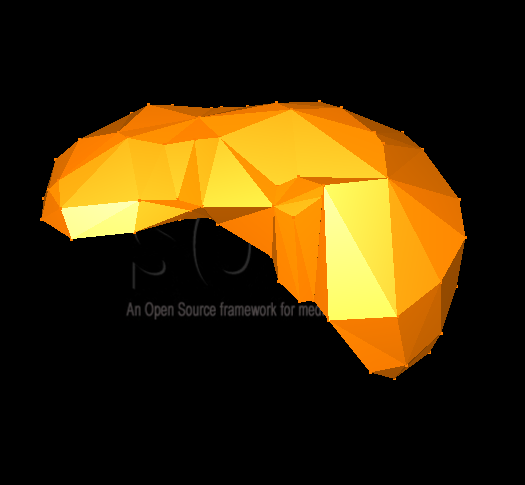
\includegraphics[width=0.4\linewidth]{liver_collision_triangles.png}
\end{figure}
\begin{itemize}
 \item same mechanical model
 \item various collision models
\end{itemize}
\end{frame}


\begin{frame}
 \frametitle{Example of interacting bodies}
Rigid and deformable bodies connected.
\begin{itemize}
 \item We attach a point to the rigid body using a mapping
 \item We insert a spring between this point and the string
\end{itemize}
\begin{figure}
 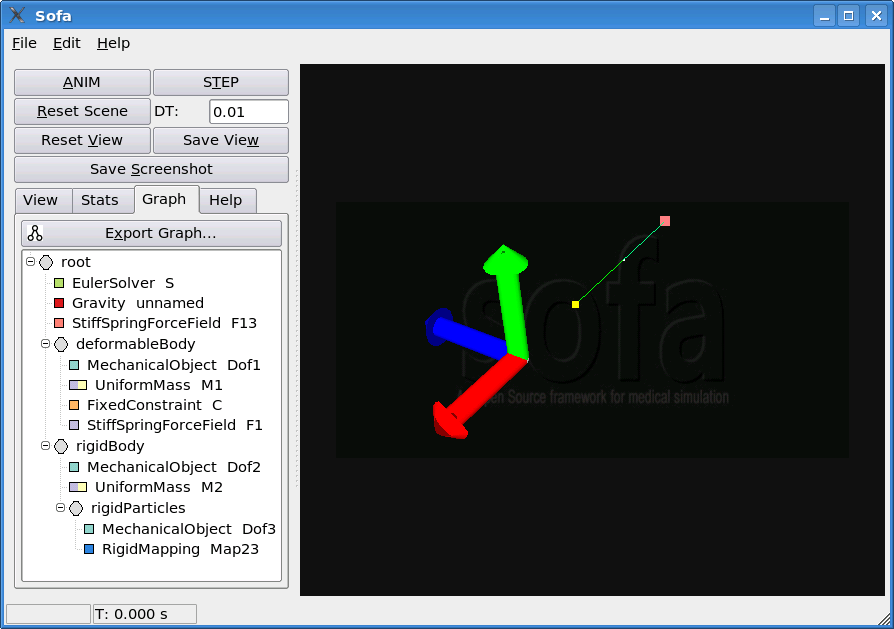
\includegraphics[width=0.8\linewidth]{mixedPendulum.png}
\end{figure}
\end{frame}

\begin{frame}
 \frametitle{A more complete picture of the scene graph}
\begin{itemize}
 \item The graph displayed in the GUI shows only the hierarchy
 \item Additional pointers are used: \end{itemize}
\begin{figure}
 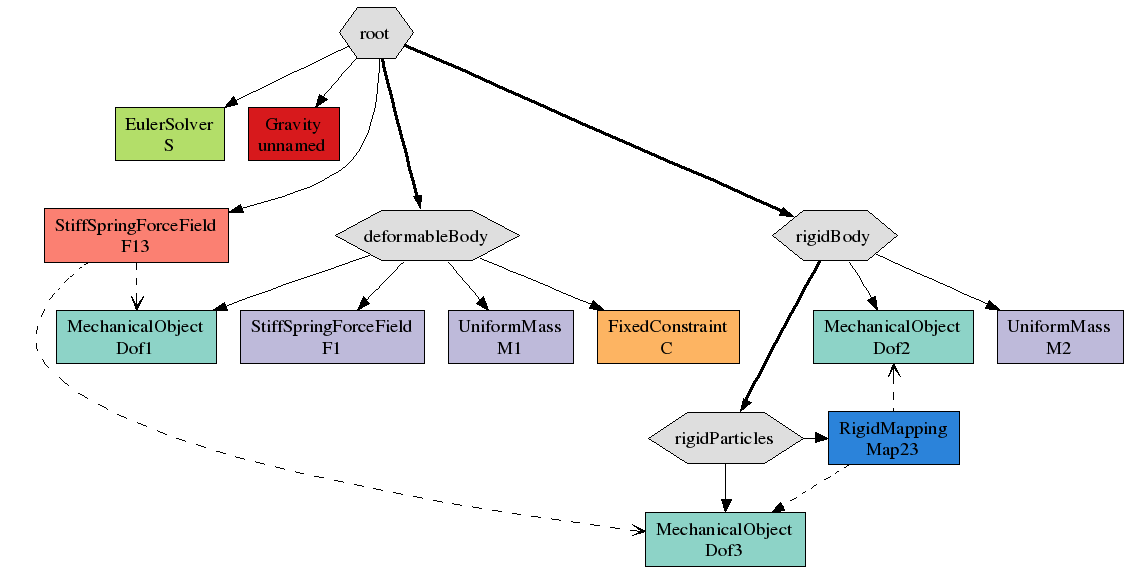
\includegraphics[width=0.99\linewidth]{mixedPendulum-graph.png}
\end{figure}
\end{frame}


% \begin{frame}
% \frametitle{Interacting bodies}
% Without interaction force
% \begin{figure}
% \begin{tabular}{c}
%  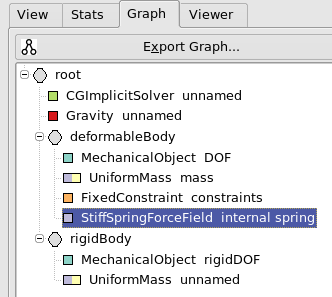
\includegraphics[height=3cm]{mixed3.png} \\ scene graph
% \end{tabular}
% \begin{tabular}{c}
%  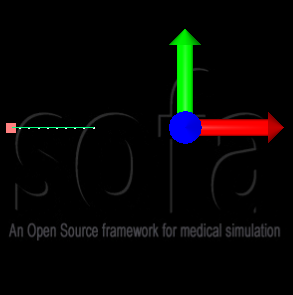
\includegraphics[height=3cm]{mixed1.png} \\ t=0
% \end{tabular}
% \begin{tabular}{c}
%  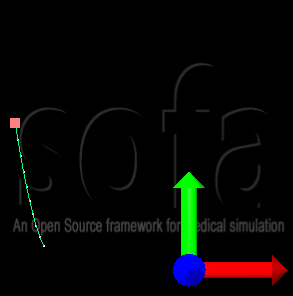
\includegraphics[height=3cm]{mixed2.png} \\ t = ...
% \end{tabular}
% \end{figure}
% \end{frame}


\begin{frame}
\frametitle{Simulation using implicit time integration}
With interaction force
\begin{figure}
\begin{tabular}{c}
 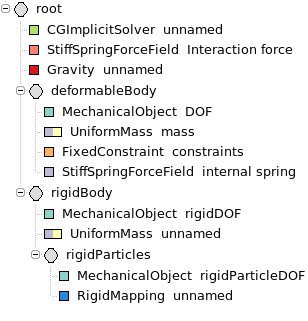
\includegraphics[height=3.7cm]{mixed11.png} \\ scene graph
\end{tabular}
\begin{tabular}{c}
 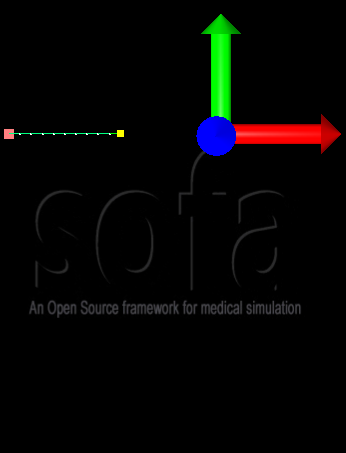
\includegraphics[height=3.7cm]{mixed9.png} \\ t=0
\end{tabular}
\begin{tabular}{c}
 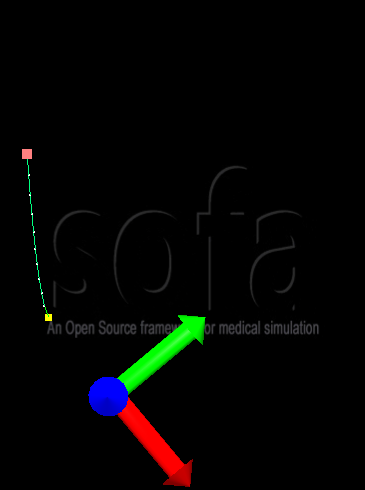
\includegraphics[height=3.9cm]{mixed10.png} \\  t = ...
\end{tabular}
\end{figure}
\end{frame}






\begin{frame}
 \frametitle{Data processing}
Sofa Visitors:
\begin{itemize}
 \item The scene graph is recursively traversed top-down and bottom-up
 \item Callbacks are applied to components of certain classes
 \item Used for all operations: physical computations, vector operations, collision detection,...
 \item Example: accumulate forces
   \begin{itemize}
    \item top-down: masses and force fields accumulate force
    \item bottom-up: mappings dispatch forces to their parents
   \end{itemize}

\end{itemize}

\end{frame}


\begin{frame}
 \frametitle{Example of visitor}
\begin{itemize}
 \item Accumulate forces, top-down callbaks:
\begin{itemize}
 \item masses accumulate their weight
 \item force fields (springs) accumulate their force
\end{itemize}
 \item each force is applied to the local Degrees of Freedom (DOF)
 \item except the interaction force
\end{itemize}

\begin{center}
 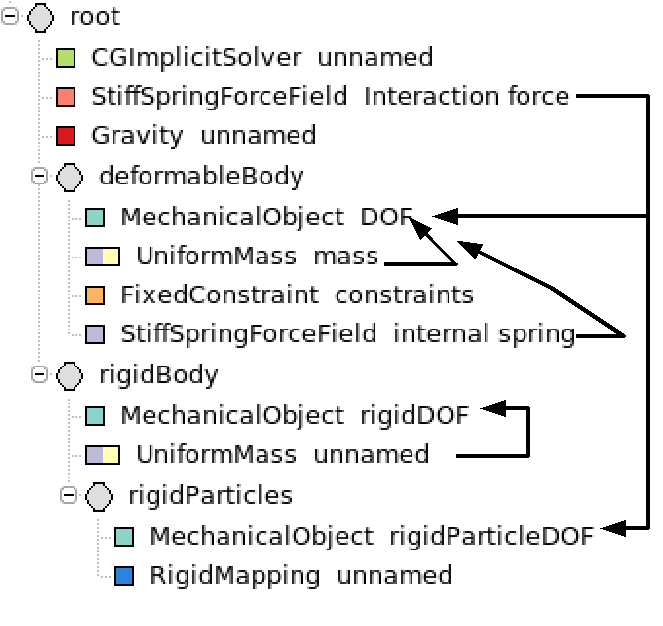
\includegraphics[width=0.37\linewidth]{slides-fig-ftopdown}
 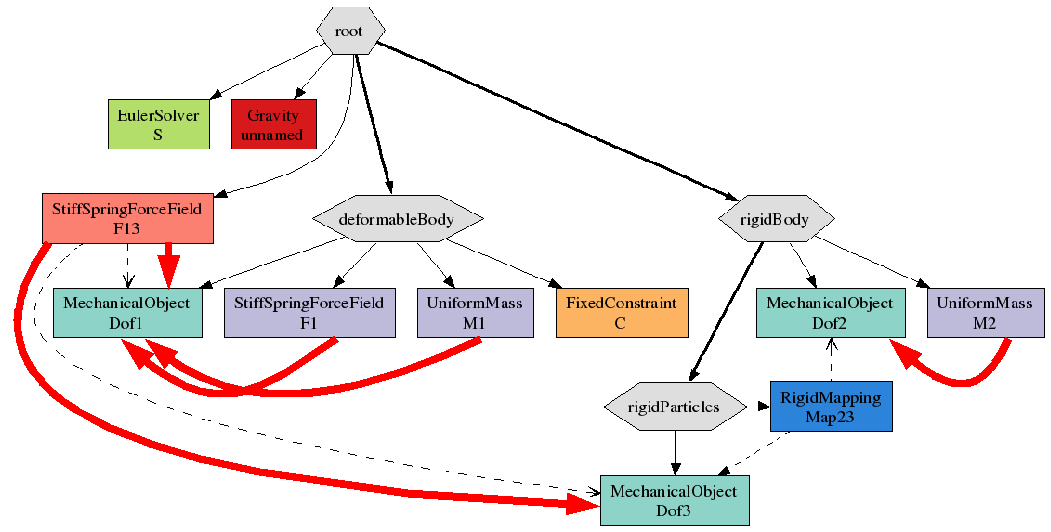
\includegraphics[width=0.57\linewidth]{slides-fig-ftopdown-dot}
 % slides-fig-ftopdown.: 1179648x0 pixel, 0dpi, infxnan cm, bb=
\end{center}

\end{frame}


\begin{frame}
 \frametitle{Example of visitor (continued)}

\begin{itemize}
 \item Accumulate forces, bottom-up callbacks:
\begin{itemize}
 \item mappings accumulate force from child to parent
\end{itemize}
 \item At the end, the net force applied to the independent (i.e. non-mapped) DOF is computed.
\end{itemize}
\begin{center}
 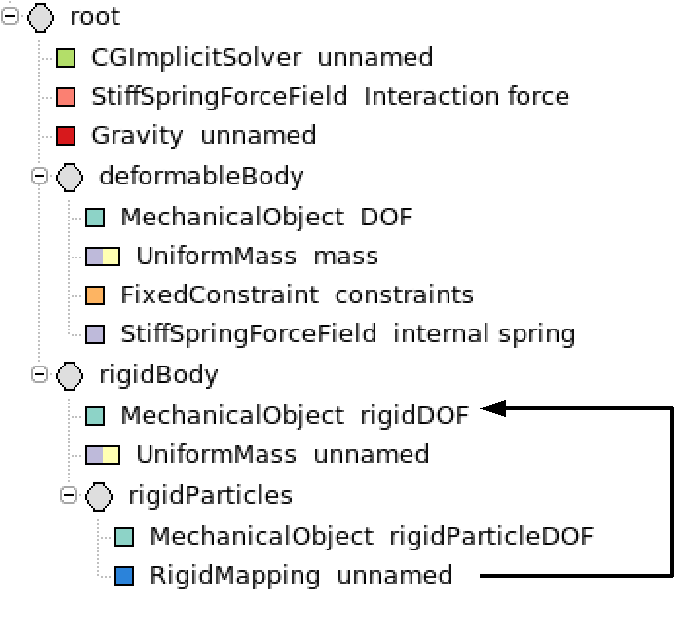
\includegraphics[width=0.37\linewidth]{slides-fig-fbottomup}
 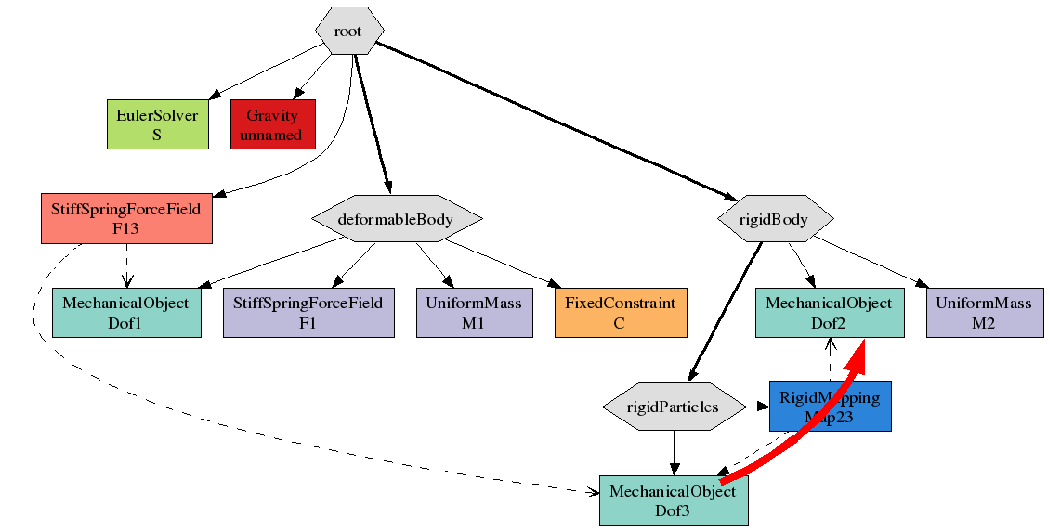
\includegraphics[width=0.57\linewidth]{slides-fig-fbottomup-dot}
\end{center}

\end{frame}


\begin{frame}
 \frametitle{Another visitor}
\begin{itemize}
 \item Compute acceleration, top-down callbacks:
\begin{itemize}
 \item masses compute $M^{-1}f$
\end{itemize}
\item modularity: uniform or diagonal (or matrix-) masses
\end{itemize}
\begin{center}
 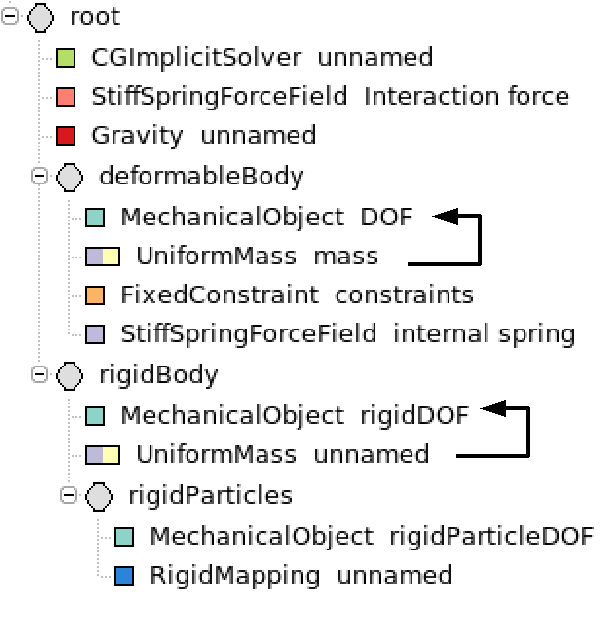
\includegraphics[width=0.37\linewidth]{slides-fig-accFromF}
 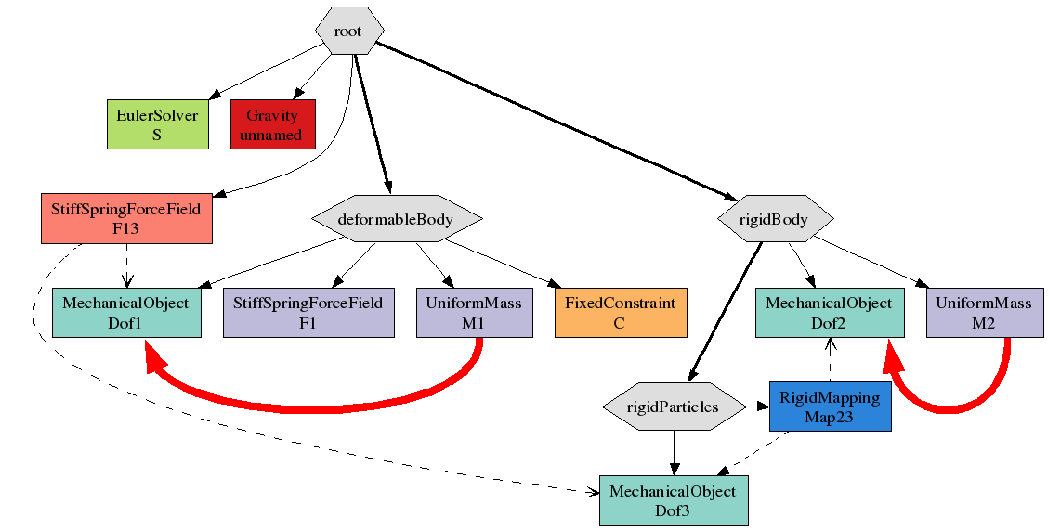
\includegraphics[width=0.57\linewidth]{slides-fig-accFromF-dot}
\end{center}

\end{frame}


\begin{frame}[fragile]
 \frametitle{Abstract state vectors}
\begin{itemize}
 \item Reserved indices are used to denote x,v,f,dx
 \item Auxiliary vectors can be used, e.g. in Runge-Kutta2:
\end{itemize}
\begin{code_cpp}
    // Allocate auxiliary vectors 
    MultiVector acc(this, VecId::V_DERIV);
    MultiVector newX(this, VecId::V_COORD);
    MultiVector newV(this, VecId::V_DERIV);

    // Compute state derivative. vel is the derivative of pos  
    computeAcc (startTime, acc, pos, vel); // acc is the derivative of vel 

    // Perform a dt/2 step along the derivative
    newX = pos;
    newX.peq(vel, dt/2.); // newX = pos + vel dt/2
    newV = vel;
    newV.peq(acc, dt/2.); // newV = vel + acc dt/2

    // compute the midpoint derivative
    computeAcc ( startTime+dt/2., acc, newX, newV);
    
    // use the midpoint derivative for the whole time step
    pos.peq(newV,dt);
    vel.peq(acc,dt);
\end{code_cpp}
\end{frame}

\begin{frame}[fragile]
 \frametitle{Degrees of Freedom (DOF)}
\begin{itemize}
 \item can be of different types (particles/rigids, float/double, ...)
 \item are stored in template class \texttt{MechanicalObject<DataType>}
 \item example of DataType (simplified):
\begin{code_cpp}
class Vec3fTypes
{
  public:
  // Basic data
      typedef float        Real;
      typedef Vec<3,float> Coord; // coordinates 
      typedef Vec<3,float> Deriv; // all the rest: velocities, forces,...

  // Data containers
      typedef vector<Real>  VecReal;
      typedef vector<Coord> VecCoord;
      typedef vector<Deriv> VecDeriv;
};
\end{code_cpp}
\item \texttt{Coord} differs from \texttt{Deriv} in 6-dof rigid bodies
\end{itemize}
\end{frame}


\begin{frame}
 \frametitle{State vectors containers}
\begin{itemize}
 \item Due to different DataTypes, the state vectors (x,v,f,a,aux,...) are scattered in the MechanicalObjects
 %\begin{center}
 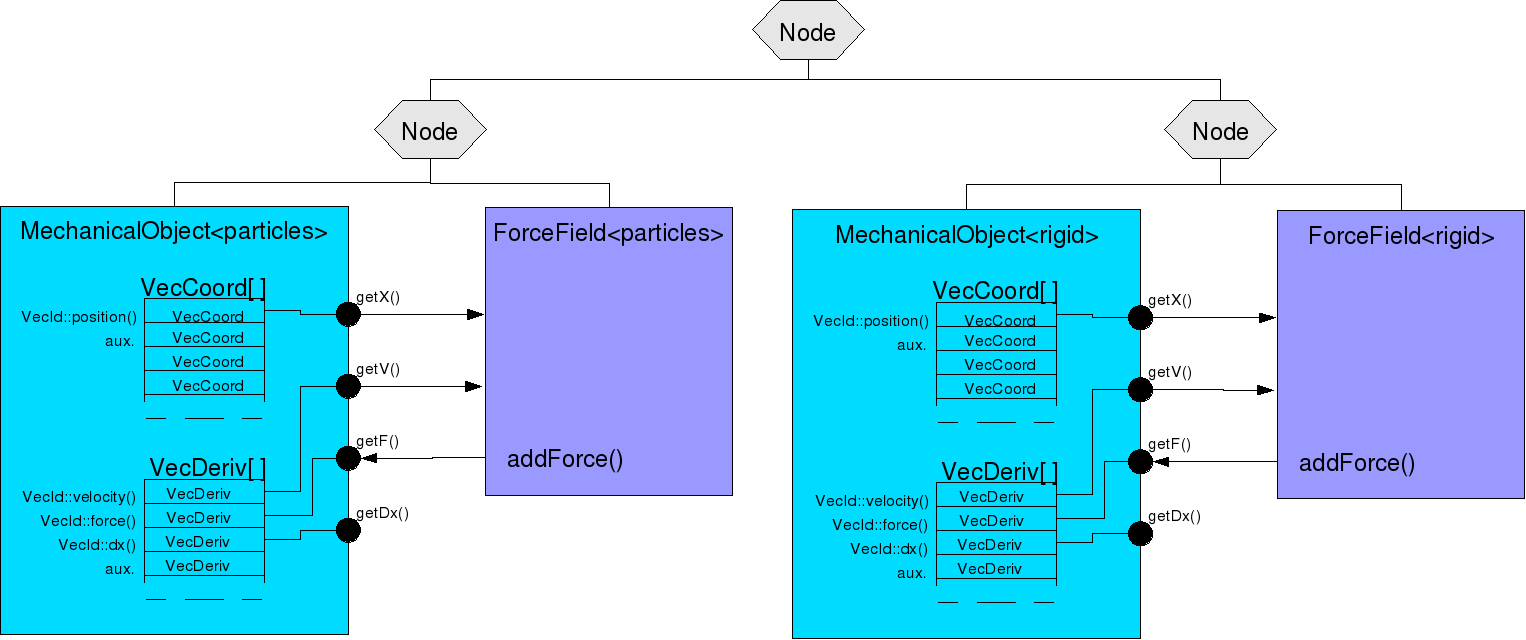
\includegraphics[width=1.1\linewidth]{MechanicalObject-particle-rigid}
%\end{center}
\item A MultiVector is a union of state vectors with a common index
\item Standard vector mathematics is implemented (sums, dot products...)
\item But no [],size(),begin(),end()
\end{itemize}

\end{frame}



\begin{frame}
 \frametitle{Control}
Simulation::init()
\begin{itemize}
 \item InitVisitor
\end{itemize}


Simulation::animate()
\begin{itemize}
 \item AnimateVisitor::processNodeTopDown
	\begin{itemize}
	 \item if MasterSolver:
		\begin{itemize}
		 \item process MasterSolver
		 \item return
		\end{itemize}
         \item process CollisionPipeline
	 \item if OdeSolvers
	\begin{itemize}
	 \item process each OdeSolver
	 \item propagate position and velocity
	 \item return
	\end{itemize}

	\item traverse children nodes
		 
	 
	\end{itemize}

\end{itemize}
\end{frame}


% \begin{frame}
%  \frametitle{Algorithms}
% At each time step:
% \begin{enumerate}
%  \item Collisions are modeled by springs using a CollisionVisitor
%  \item Differential Equation solvers update x and v 
%  \item Mappings propagate the new state to all the layers and external buffers (rendering)
% \end{enumerate}
% ODE solvers and collision modeling modules are easily customizable.
% \end{frame}


\begin{frame}
 \frametitle{Conclusion}
Strengths:
\begin{itemize}
 \item Interaction of multiple models using mappings
 \item Efficient simulation of deformable bodies using implicit time integration
 \item Highly customizable
\end{itemize}
Weaknesses:
\begin{itemize}
 \item Documentation
 \item Multiple control layers (need to simplify this)
\end{itemize}
Ongoing work:
\begin{itemize}
 \item Parallelisation (clusters, and more GPU)
 \item Constraint-based methods 
 \item Traces and profiling
\end{itemize}

\end{frame}







\end{document}
